% ****** Start of file aipsamp.tex ******
%
%   This file is part of the AIP files in the AIP distribution for REVTeX 4.
%   Version 4.1 of REVTeX, October 2009
%
%   Copyright (c) 2009 American Institute of Physics.

\documentclass[
 aip,
 jmp,
 amsmath,amssymb,
%preprint,
 reprint,
%author-year,
%author-numerical,
]{revtex4-1}

\usepackage{graphicx}
\usepackage{grffile}
\usepackage{dcolumn}
\usepackage{bm}
%\usepackage[mathlines]{lineno}% Enable numbering of text and display math
%\linenumbers\relax % Commence numbering lines
\usepackage{multirow}
\usepackage{color}

\begin{document}

\preprint{AIP/123-QED}

\title[Musimetrics]{Musimetrics}

\author{Vilson Vieira}%
 \homepage{http://automata.cc}
 \email{vilson@void.cc}

\author{Renato Fabbri}%
 \homepage{http://www.estudiolivre.org/el-user.php?view\_user=gk}
 \email{renato.fabbri@gmail.com}

\author{Luciano da Fontoura Costa}
  \homepage{http://cyvision.ifsc.usp.br/~luciano/}
  \email{ldfcosta@gmail.com}
  \affiliation{ 
Instituto de F\'isica de S\~ao Carlos, Universidade de S\~ao Paulo (IFSC/USP)
}

\date{\today}

\begin{abstract}

Based on a quantitative philosophical analysis,
we verified the application of same method to another field of knowledge: music. Seven
composers of classical music were analyzed with respect of
eight main musical characteristics present on their life-work.
In addition, both philosophical and musical analysis
were compared, revealing some differences on the development of
each of these fields, specially with respect to innovation.

\end{abstract}

\pacs{89.75.Fb,05.65.+b}% PACS, the Physics and Astronomy
\keywords{music, musicology, pattern recognition, statistics}

\maketitle

\section{\label{sec:level1}Introduction}

Along the history of music, composers developed their own styles along a
continuous search for coherence or unity. In the words of Anton
Webern~\cite{Webern}, ``[...] ever since music has been written most great artists
have striven to make this unity ever clearer. Everything that has
happened aims at this [...]''. On this process we could argue that
inheritance of style from one composer to another is constantly
present, as noted by William Lovelock~\cite{Lovelock}:
``[...] it [a new style of writing] is a gradual development from its
predecessor, in due course reaching its culmination, and germinating
in its life the seeds of its successor'', contrasting with the
necessity of innovation, also cited by the same author: 
``It is only by experiment that progress is possible; it is the man
with the forward-looking type of mind [...] who forces man out of the
rut of 'what was good enough for my father is good enough for me'.''
How innovation is shown in
this master-apprentice context? How the quest for coherence is
developed by composers considering this dichotomy?

Other fields of knowledge -- like philosophy -- demonstrate
a well-defined trend when considering innovation: the
quest for difference seems to drive philosophical
changes~\cite{Deleuze}. Recently, this observation became more evident with
the application of quantitative analysis~\cite{Fabbri}: a series of statistical
and pattern recognition steps that create a formal representation of
the philosophical movements along the history. More specifically, the method consists of
scoring memorable philosophers based on some dualistic
characteristics. The group of philosophers was choose
based on the historical relevance of each philosopher. The
scores assigned to each philosopher compose a state
vector in complex space. The application
of Pearson correlation reveals the most important relations between
the issues and principal component analysis (PCA) makes possible to
represent the philosophical history as a planar graph where we could
identify interesting properties. Even argument based methods like dialectics
seem to be well modeled as mathematical relations between the
philosophical states. Following this work we
expanded the analysis in order to better understand how
innovation evolved in music and how it is compared to
philosophy where opposition was identified as a strong factor
concerning innovation and dialectics .

The application of statistical analysis to classical
music is not recent. On musicology, statistical methods have been used
to identify many musical characteristics.
Simonton~\cite{Simonton1991829, Simonton1977791}, beyond several
works, used time-series analysis to measure the creative productivity
of composers based on its produced musics and popularity. Kozbelt~\cite{Kozbelt01012009, Kozbelt01012007} also
analysed the productivity, but based on the measure of performance
time of the compositions and investigated the relation between
productivity and versatility. More recent works~\cite{Kranenburg2004, Kranenburg2007} uses machine-learning
algorithms to recognize musical styles of selected compositions.

Differently from these works, we are not interested in applying
statistical analysis to music but on characterizing concerning composers.
We chose seven memorable composers from different periods of classical music.
Eight characteristics were described and scored by the authors, based
on the recurrent appearance of these issues in music pieces composed
by the selected musicians. The same statistical method developed for
philosophy was applied to this set of composers and their
characteristics, making possible to compare the results on both areas.

We start by describing how the original method was adapted to the
analysis of composers. The eight musical characteristics are 
discussed as the composers and their respective musical period,
followed by results and comparisons between the application of the
method on philosophy and music.

\section{Mathematical Description}

A set of music composers was chosen based on their
relevance as representatives of each period of the classical music history.
A sequence $S$ of $P$ composers include the $P$ most visible composers
in that time interval. Because this time interval vary on each period,
the sequence $S$ does not necessarily corresponds to an uniform time series.

As done for philosophers~\cite{Fabbri}, the set of $C$ measurements
define a $C-$dimensional space referred as the \emph{musical space}.  
The characteristic vector $\vec{v_i}$ of each composer $i$ defines a respective
\emph{composer state} in the musical space.  

For the set of
$P$ composers, we used the same elements defined for philosophers
~\cite{Fabbri}: \emph{average state at time $i$}, named $\vec{a_i}$;
the \emph{opposite state} of a given composer state $\vec{v_i}$, named $\vec{r_i}$;
the \emph{opposition vector} of composer state $\vec{v_i}$, named
$\vec{D_i}$; and the \emph{opposition
amplitude} of that same state, $|| \vec{D_i} ||$.

The dialectics is quantified between a triple of successive composers
 $i, j$ and $k$ of the given set $P$. This makes possible to examine whether
the dialectics remains an interesting relation between music composers like it was
for philosophers.

\section{Musical Characteristics}

To create the musical space we derived eight variables corresponding to
distinct characteristics commonly found on music compositions. The
characteristics are related with the basic elements of music -- melody,
harmony, rhythm, timbre, form and tessitura~\cite{BennettHistory} -- and
non-musical issues like historical events that have influenced the
compositions, for example, the
presence of Church along the early development of music. All the eight
characteristics are listed below:

{\bf \em{ Sacred - Secular}} (\emph{S-P}): the sacred or religious music is
composed through religious influence or used for its purposes. \textit{Masses},
\textit{Motets} and hymns, dedicated to the Catholic liturgy, are well known examples~\cite{Lovelock}. Secular
music is its opposite, having no relation with religion, also known as
popular songs like Italian madrigals and German \textit{Lieds}~\cite{BennettHistory}. 

{\bf \em{ Short duration - Long duration}} (\emph{S-L}): compositions are
quantified having short duration when it does not have more than few minutes
of execution. Long duration compositions have at least 20 minutes of execution or
more. The same consideration was did by Kozbelt~\cite{Kozbelt01012009,
  Kozbelt01012007} with his analysis of time execution.

{\bf \em{ Harmony - Counterpoint}} (\emph{H-C}): harmony emphasizes the harmonic
discourse, considering the priority use of just one single melody,
contrasting with counterpoint, which Bach's fugues are the better examples~\cite{BennettHistory}.

{\bf \em{ Vocal - Instrumental}} (\emph{V-I}): compositions using just vocals
(e.g. \emph{cantata}) or exclusively instruments
(e.g. \emph{sonata}). It is interesting to note the use supreme of
vocals over instruments on Sacred compositions~\cite{Lovelock}.

{\bf \em{ Non-discursive - Discursive}} (\emph{N-D}): compositions
based or not
on verbal discourse, like programmatic music or Baroque rhetoric, where the composer wants
to ``tell a history'' invoking images to the listeners
mind~\cite{BennettHistory}. Its contrary part is known as
\textit{absolute music} where the music is written to be appreciated simply
by what it is.

{\bf \em{ Motivic Stability - Motivic Variety}} (\emph{M-V}): motivic pieces presents equilibrium
between repetition, reuse and variation of melodic motives. The other vary the use of new
materials along the composition. Bach is noticeable by his
\textit{development by variation} of motives, contrasting with the
constantly inventive use of new materials by Mozart~\cite{Webern}.

{\bf \em{ Rhythmic Simplicity - Rhythmic Complexity}} (\emph{R-P}): presence or not of polyrhythms, the
use of independent rhythms at the same time -- also known as
\textit{rhythmic counterpoint}\cite{BennettHistory} -- a characteristic
constantly found on the works of 20th-century composers like Stravinsky.

{\bf \em{ Harmonic Stability - Harmonic Variety}} (\emph{T-M}):
rate of tonality change on a piece or its stability. After the highly
polyphony development in Renaissance, Beethoven is credited as the
composer who returned to the maximum exploration of harmonic variety~\cite{Webern}.

\section{Results and Discussion}

Memorable composers were chosen as key representatives
of the musical development. The set
is ordered chronologically and presented on Table \ref{tab:table0} with
each composer related with its historical period.

\begin{table}[ht]
\caption{\label{tab:table0} The set of music composers ordered chronologically
with the outstanding period their represents.}

\begin{tabular}{|l||l|}
\hline

 Composers       &  Eras \\ \hline

 Monteverdi      & Renaissance \\
 Bach            & Baroque \\
 Mozart          & Classical \\
 Beethoven       & Classical $\to$ Romantic \\
 Brahms          & Romantic \\
 Stravinsky      & 20th-century \\
 Stockhausen     & Contemporary\\

\hline
\end{tabular}
\end{table}

The quantification of the eight musical
characteristics was performed jointly by the authors of this
article and is shown in Table \ref{tab:tableA}. The scores were
numerical values between 1 and 9. Values more close of 1 reveals the
composer tended to the first element of each characteristic pair and
vice versa. It is important to note the efficiency of this method
concerning possible errors due to a subsequent perturbation of
original scores. If this initial step of analysis was susceptible to
errors, all the proposed work would be bound to failure. This
perturbation method is better explained in this section.

\begin{table}[ht]
\caption{\label{tab:tableA}Quantification of the
eight music characteristics for each of the seven composers.}

\begin{ruledtabular}
\begin{tabular}{|l||c|c|c|c|c|c|c|c|}

 Composers    & S-P & S-L & H-C & V-I & N-D & M-V & R-P & T-M  \\
\hline
 Monteverdi   & 3.0 & 8.0 & 5.0 & 3.0 & 7.0 & 5.0 & 3.0 & 7.0  \\
 Bach         & 2.0 & 6.0 & 9.0 & 2.0 & 8.0 & 2.0 & 1.0 & 5.0  \\
 Mozart       & 6.0 & 4.0 & 1.0 & 6.0 & 6.0 & 7.0 & 2.0 & 2.0  \\
 Beethoven    & 7.0 & 8.0 & 2.5 & 8.0 & 5.0 & 4.0 & 4.0 & 7.0  \\
% Chopin & 9.0 & 3.0 & 3.0 & 9.0 & 5.5 & 8.0 & 7.0 & 8.0 \\
 Brahms       & 6.0 & 6.0 & 4.0 & 7.0 & 4.5 & 6.5 & 5.0 & 7.0  \\
 Stravinsky   & 8.0 & 7.0 & 6.0 & 7.0 & 8.0 & 5.0 & 8.0 & 5.0  \\
 Stockhausen  & 7.0 & 4.0 & 8.0 & 7.0 & 5.0 & 8.0 & 9.0 & 6.0  \\

\end{tabular}
\end{ruledtabular}
\end{table}

This data set defines an 8-dimensional musical space, each dimension
corresponding of one characteristic. The
Pearson correlation coefficients between the eight musical
characteristics chosen are presented in Table \ref{tab:tableB}.
The coefficients with absolute value larger than 0.5 are emphasized.

\begin{table}[ht]
\caption{\label{tab:tableB}Pearson correlation coefficients between
  the eight musical characteristics.}

\begin{ruledtabular}
\begin{tabular}{|c||c|c|c|c|c|c|c|c|}

-   &  S-P  &  S-L  &  H-C    &  V-I   &  N-D    &  M-V           &  R-P            &  T-M  \\ \hline
S-P & -     &  -0.16 &  -0.35 &  \textbf{0.95}  &  -0.43  &  \textbf{0.56}   &  \textbf{0.74}   &  -0.05 \\
S-L & -     &  -     &  -0.07 &  -0.12 &  0.26  &  \textbf{-0.61}  &  -0.15  &  \textbf{0.63} \\
H-C & -     &  -     &  -     &  -0.45 &  0.43  &  -0.29  &  0.27   &  0.25 \\
V-I & -     &  -     &  -     &  -     &  \textbf{-0.65} &  \textbf{0.55}   &  \textbf{0.64}   &  0.09 \\
N-D & -     &  -     &  -     &  -     &  -     &  \textbf{-0.61}  &  -0.24  &  -0.3 \\
M-V & -     &  -     &  -     &  -     &  -     &  -      &  \textbf{0.55}   &  -0.16 \\
R-P & -     &  -     &  -     &  -     &  -     &  -      &  -      &  0.27 \\
T-M & -     &  -     &  -     &  -     &  -     &  -      &  -      &  - \\

\end{tabular}
\end{ruledtabular}
\end{table}

We can identify some interesting relations between the pairs of
characteristics that reflect important facts found on music history. For
instance, the Pearson correlation coefficient of 0.95 was obtained for
the pairs S-P (Sacred or Secular) and V-I (Vocal or Instrumental), which indicates sacred music is more vocal then
instrumental. The coefficient of 0.74 also shows it does not commonly use polyrhythms as we can see
analysing the pairs S-P and R-P (Rhythmic Simplicity or Complexity).
Negative coefficients indicate the contrary direction like the
value of -0.65 of the pairs V-I and N-D (Non-discursive or Discursive) indicating composers that used
just voices on their compositions also preferred to use programmatic
musics techniques like baroque rhetoric.
To reduce the number of dimensions -- making possible to visualize the
musical space as a planar graph, filtering just the relevant
characteristics -- PCA was applied to this set of data, yielding the new variances given
in Table \ref{tab:tableC} in terms of percentages of total
variance. We can note the concentration of variance along the two
first PCA axes, a common effect also examined while analysing
philosophers characteristics~\cite{Fabbri}. This means we could
consider just two dimensions, yielding a planar
musical space.

\begin{table}[ht]
\caption{\label{tab:tableC}New variances after PCA, in percentages for
  scores on \ref{tab:tableB}.}

\begin{tabular}{|c||c|}
\hline
Eigenvalue  & Value     \\ \hline

$\lambda_1$ &  45.62 \% \\
$\lambda_2$ &  22.32 \% \\
$\lambda_3$ &  17.32 \% \\
$\lambda_4$ &  11.09 \% \\
$\lambda_5$ &   3.62 \% \\
$\lambda_6$ &   0.26 \% \\
$\lambda_7$ &   0.   \% \\
\hline

\end{tabular}
\end{table}

As done for philosophers analysis, we performed 1000 perturbations of
the original scores by adding the values -2, -1, 0, 1 and 2 with
uniform probability. In other words, we wanted to test if scoring
errors could be sufficient to cause relevant effects
on the PCA projections. Interestingly, the values of average and
standard deviation for both original and perturbed positions listed on Table
\ref{tab:tableD} show relatively small perturbations. It is therefore
reasonable to say small errors in the values assigned as scores of composers
characteristics did not affected too much its quantification.

%% perturbacoes

\begin{table}%\footnotesize%\scriptsize%\tiny
\caption{\label{tab:tableD}Average and standard deviation of the 
deviations for each composer and for the first 
4 eigenvalues.}

% \begin{ruledtabular}
\begin{tabular}{|c||c|c|}
\hline

Composers & $\mu_{\Delta}$ & $\sigma_{\Delta}$ \\
\hline

Monteverdi     & 1.5398 & 0.8598 \\
Bach           & 1.2971 & 0.8858 \\
Mozart         & 3.2419 & 1.9023 \\
Beethoven      & 1.8649 & 1.0310 \\
Brahms         & 1.2971 & 0.7041 \\
Stravinsky     & 1.3389 & 0.6496 \\
Stockhausen    & 1.7097 & 0.9447 \\
\hline \hline
Eigenvalues & $\mu_{\Delta}$ & $\sigma_{\Delta}$ \\
\hline
$\lambda_1$ &  -0.0391 & 0.0519 \\
$\lambda_2$ &   0.0336 & 0.0343 \\
$\lambda_3$ &  -0.0034 & 0.0283 \\
$\lambda_4$ &  -0.0114 & 0.0261 \\
\hline

\end{tabular}
% \end{ruledtabular}
\end{table}

Table \ref{tab:Deviates} shows the normalized weights
of the contributions of each original property on the two
new main axes. Most of the characteristics contribute almost equally
in defining the two main axes, letting us to consider a 2-dimensional
space presented in Figure \ref{fig:pca}.

\begin{table}[ht]
\caption{\label{tab:Deviates}Percentages of
the contributions from each musical characteristic on the two
new main axes.}

\begin{tabular}{|c||c|c|}
\hline
Musical         & \multirow{2}{*}{$C_1$} & \multirow{2}{*}{$C_2$} \\
Characteristics & & \\
\hline
 S-P              &  18.46  &   4.30  \\
 S-L              &   7.83  &  25.56  \\
 H-C              &   8.32  &   7.72  \\
 V-I              &  19.05  &   6.57  \\
 N-D              &  14.92  &   3.38  \\
 M-V              &  16.97  &   9.58  \\
 R-P              &  14.32  &  12.28  \\
 T-M              &   0.12  &  30.60  \\
\hline
\end{tabular}
% \end{ruledtabular}
\end{table}

The arrows follow the time sequence along with the seven
composers. Each of these arrows corresponds to a musical move from one
composer state to another -- for clarity, just the lines of the arrows
are preserved. The graph shows interesting results. 

Bach, as could be expected, is positioned far from the rest of
composers. It is related of his incomparable genius, notoriously
admitted by other great composers like Beethoven and
Webern~\cite{Webern}: ``In fact Bach composed everything, concerned
himself with everything that gives food for thought!''. 
We can identify a strong relationship between
Beethoven and Brahms, reflecting the belief of the \textit{virtuosi} Hans von B\"{u}low~\cite{Bulow} when he
stated the $1^{st}$ Symphony of Brahms as, in reality, being the \textit{$10^{th}$ Symphony of
Beethoven}, clamming Brahms as the true successor of Beethoven. Stravinsky is at the center of all
relations, presumably due to his heterogeneity~\cite{BennettHistory, Lovelock}.
For Webern, Beethoven was the unique classicist who really came close
to the coherence found in the pieces of the Burgundian School: ``Not even
in Haydn and Mozart do we see these two forms as clearly as in
Beethoven. The period and the eight-bar sentence are at their purest
in Beethoven; in his predecessors we find only traces of them''~\cite{Webern}. It
could explain the proximity of Beethoven to the Renaissance  Monteverdi.
Mozart is the most deviating point in the space, even when compared with
Beethoven who was deeply influenced by Mozart, mainly in his early works. This
is possibly explained by the overly complexity of Mozart works, just influenced by his contemporary Haydn~\cite{Lovelock}.
Maybe Stockhausen could present similar detachment if we considered
more vanguard characteristics -- e.g. timbre exploration by using
electronic devices~\cite{Lovelock} -- not
shared by his precursors.
In general, the musical movements have minor opposition, and
remembering the beginning of this work, it reflects the apprentice-master
tradition present on music: the composers tend to build their own
works based on its precursor. This reveals a crucial difference
considering the \textit{memory state} along the development of
philosophy and music: while a philosopher was influenced by the
opposition of ideas of its two predecessors, composers were commonly
influenced by their direct predecessor. Therefore, we can argue that philosophy
presents a \textit{memory-2} state, while music presents
\textit{memory-1}, considering \textit{memory-N} being the number $N$
of past generations that influenced a philosopher or composer.

% Figure~\ref{fig:time} shows the two principal components in terms of
% time-slots. We can identify again the two groups of composers and the
% minor opposition between the components during its evolution.

\begin{figure}[ht]
  \begin{center}
    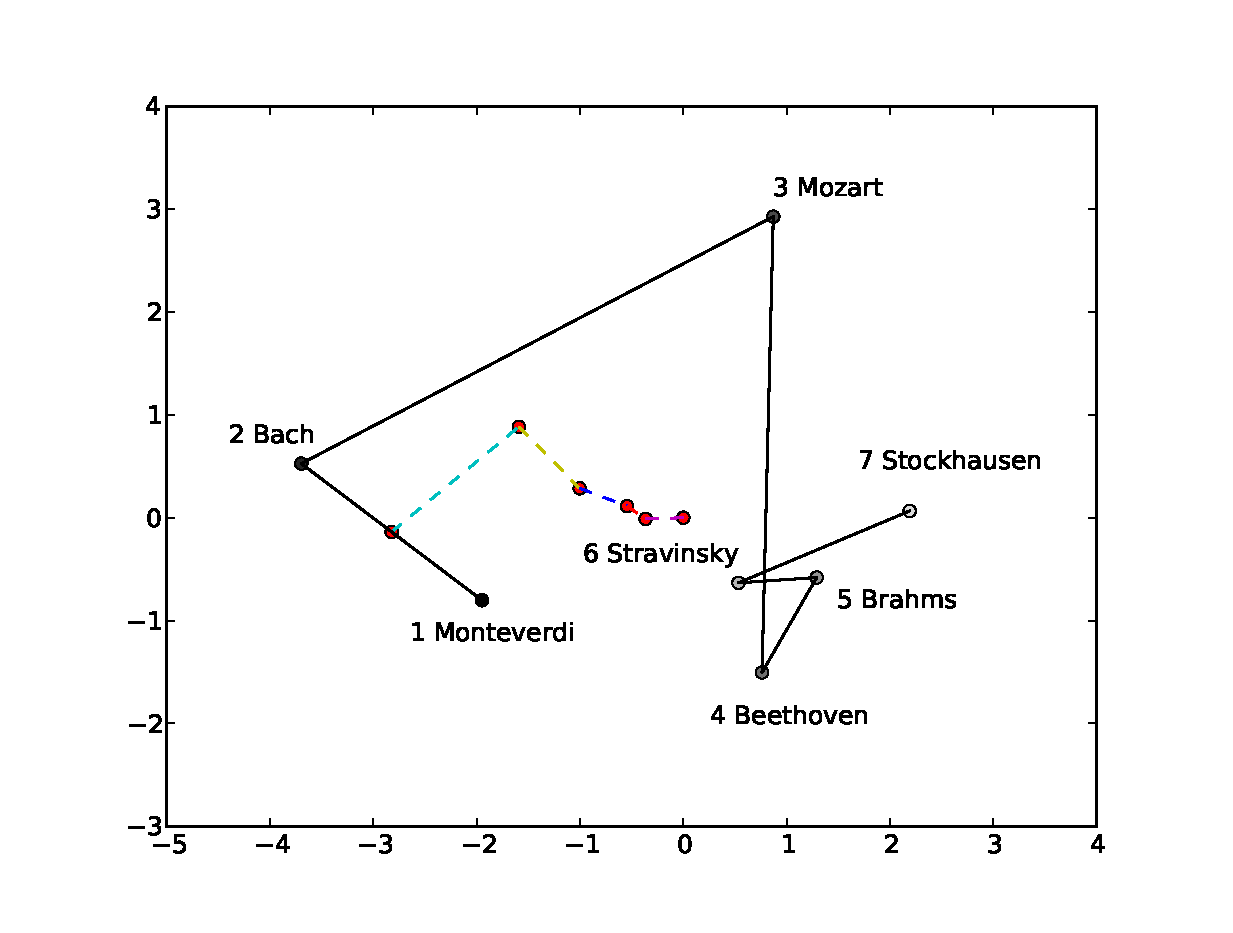
\includegraphics[width=0.45\textwidth]{images/g1}
  \end{center}
  \caption{\it 2-dimensional projected musical space.}
  \label{fig:pca}
\end{figure}

% \begin{figure}[ht]
%         \begin{center}
%                 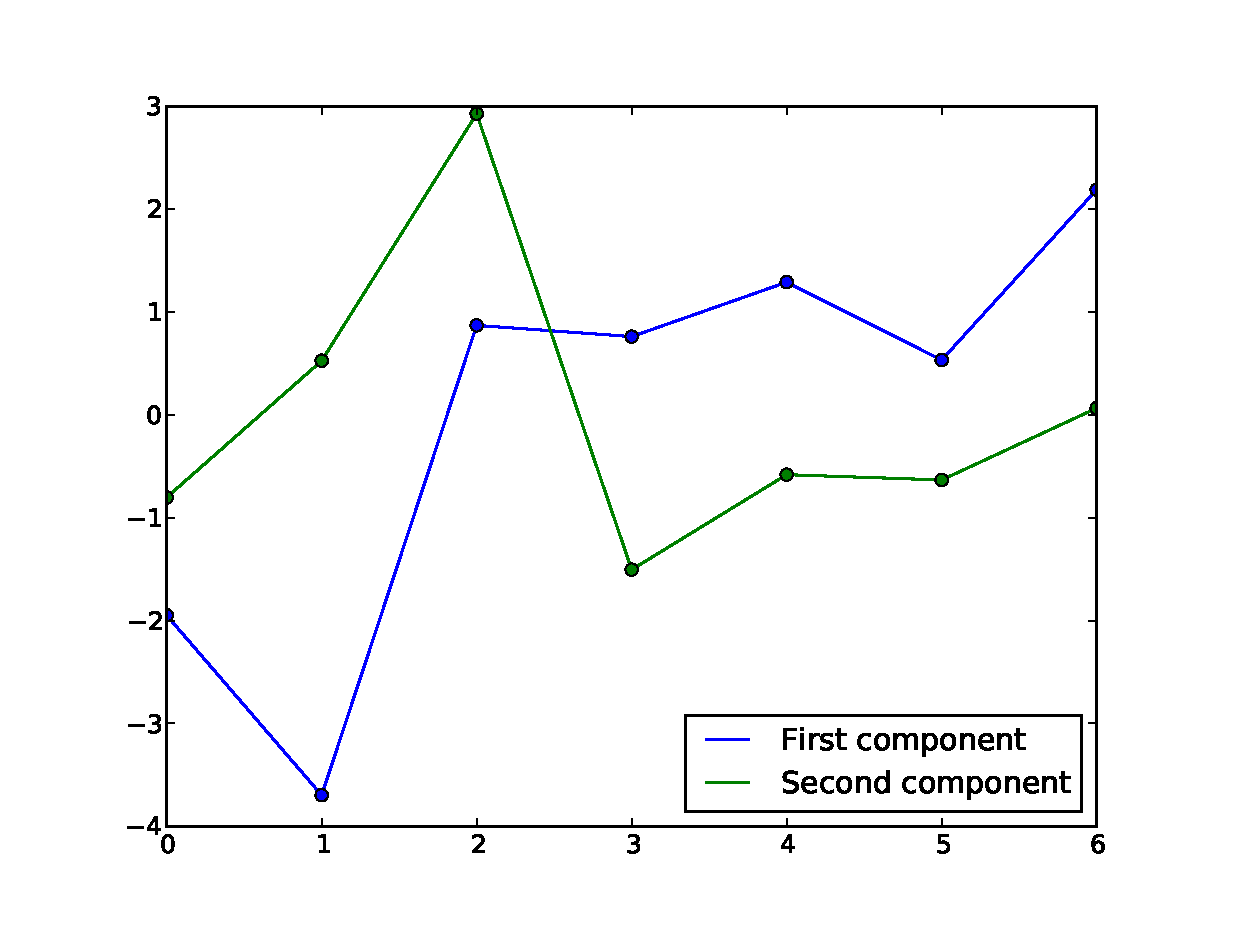
\includegraphics[width=0.45\textwidth]{images/g2}
%         \end{center}
%         \caption{\it Time evolution of the two principal components.}
%         \label{fig:time}
% \end{figure}

To complement the analysis, Table \ref{tab:tableOI} gives the
opposition and skewness indices for each of the six musical moves,
showing the movements are driven by rather small opposition and strong
skewness. In other words, most musical moves do not benefit from
opposition as far as innovation is concerned. Dialectics is also analyzed on Table
\ref{tab:tableE} where we identified an alternation of values along
the pairs of subsequent musical movements: the first value of
counter-dialectics is greater than the second, that is lesser than the
third and so on. There is no strong
dialectics, but a continuous variation.

\begin{table}[ht]
\caption{\label{tab:tableOI}Opposition and skewness indices for each
of the six musical moves.}

\begin{tabular}{|c||c|c|}
\hline
Musical Move & $W_{i,j}$ & $s_{i,j}$ \\
\hline \hline

 Monteverdi $\to$ Bach             &   1.0     &  0       \\
 Bach $\to$ Mozart                 &   1.1484  &  1.6028  \\
 Mozart $\to$ Beethoven            &   0.5679  &  2.4759  \\
 Beethoven $\to$ Brahms            &   0.0929  &  0.9919  \\
 Brahms $\to$ Stravinsky           &   0.1996  &  0.2954  \\
 Stravinsky $\to$ Stockhausen      &  -0.3224  &  1.7169  \\

\hline
\end{tabular}
\end{table}

\begin{table}[ht]
\caption{\label{tab:tableE} Counter-dialectics index for each
of the five subsequent pairs of musical moves.}

\begin{tabular}{|c||c|}
\hline
Musical Triple & $d_{i \rightarrow k}$ \\
\hline \hline

 Monteverdi $\to$ Bach $\to$ Mozart          &     0.495  \\
 Bach $\to$ Mozart $\to$ Beethoven           &     0.082  \\
 Mozart $\to$ Beethoven $\to$ Brahms         &     0.289  \\
 Beethoven $\to$ Brahms $\to$ Stravinsky     &     0.104  \\
 Brahms $\to$ Stravinsky $\to$ Stockhausen   &     1.741  \\

\hline
\end{tabular}
\end{table}

\section{Comparisons with Philosophers Analysis}

The results of composers analysis when compared with philosophers
reveals surprising results. If we compare the discussed musical space
with the philosophical one of Figure \ref{fig:phipca} we can
identify opposite movements along all the philosophy history in contrast
to music. This reveals a notorious characteristic of the way
philosophers seem to have evolved their ideas, driven by opposition, while
composers tend to inherit characteristics from the works of their
predecessors.

\begin{figure}
  \begin{center}
    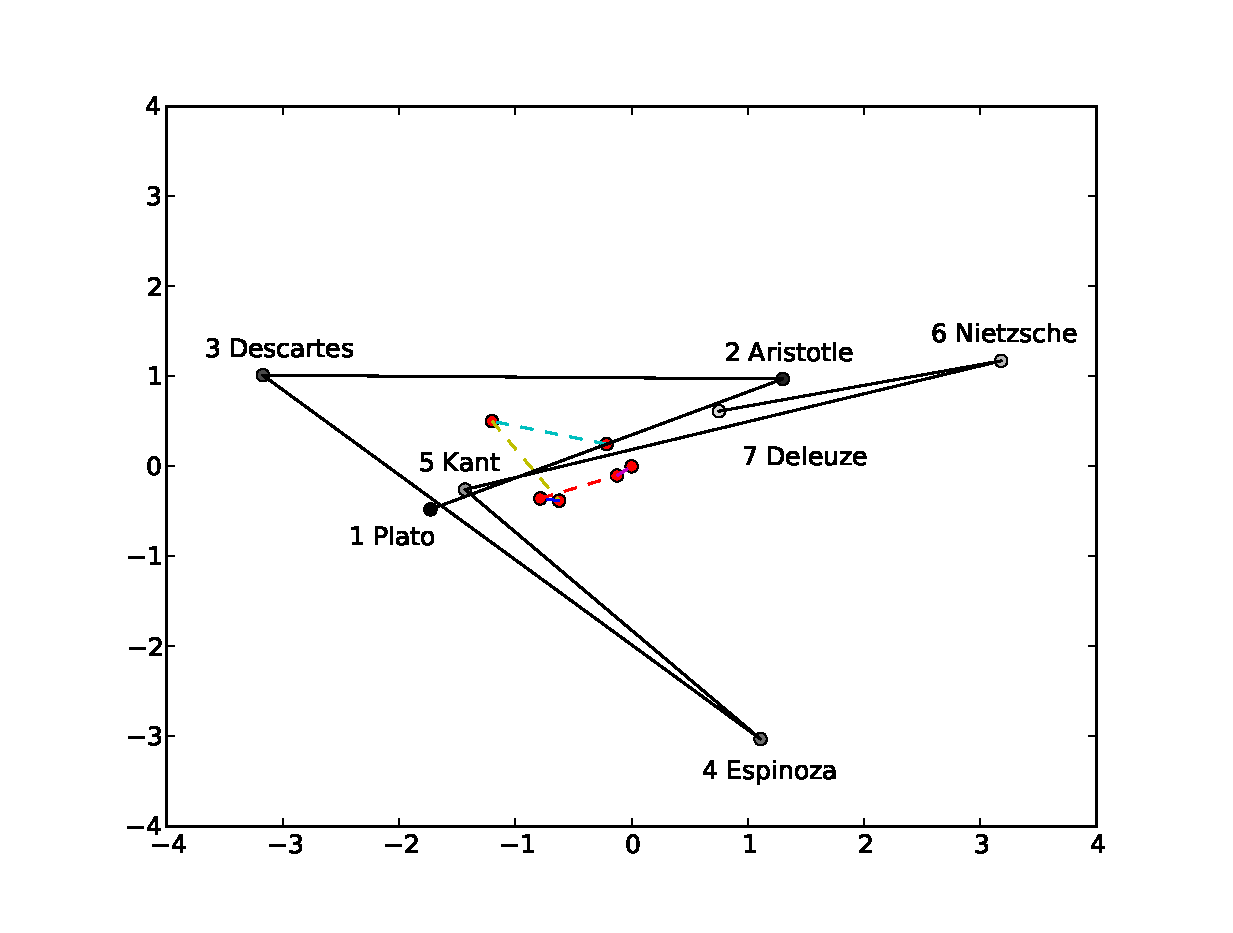
\includegraphics[width=0.45\textwidth]{images/g1filosofos}
  \end{center}
  \caption{\it 2-dimensional projected philosophical space~\cite{Fabbri}.}
  \label{fig:phipca}
\end{figure}

% Comparing the time evolution of principal components of both fields,
% we can see, as shown in Figure \ref{fig:phitime}, a well-defined
% reflection pattern between each time slot, again contrasting with the
% composers time evolution, where both components show linear movements.

% \begin{figure}
%   \begin{center}
%     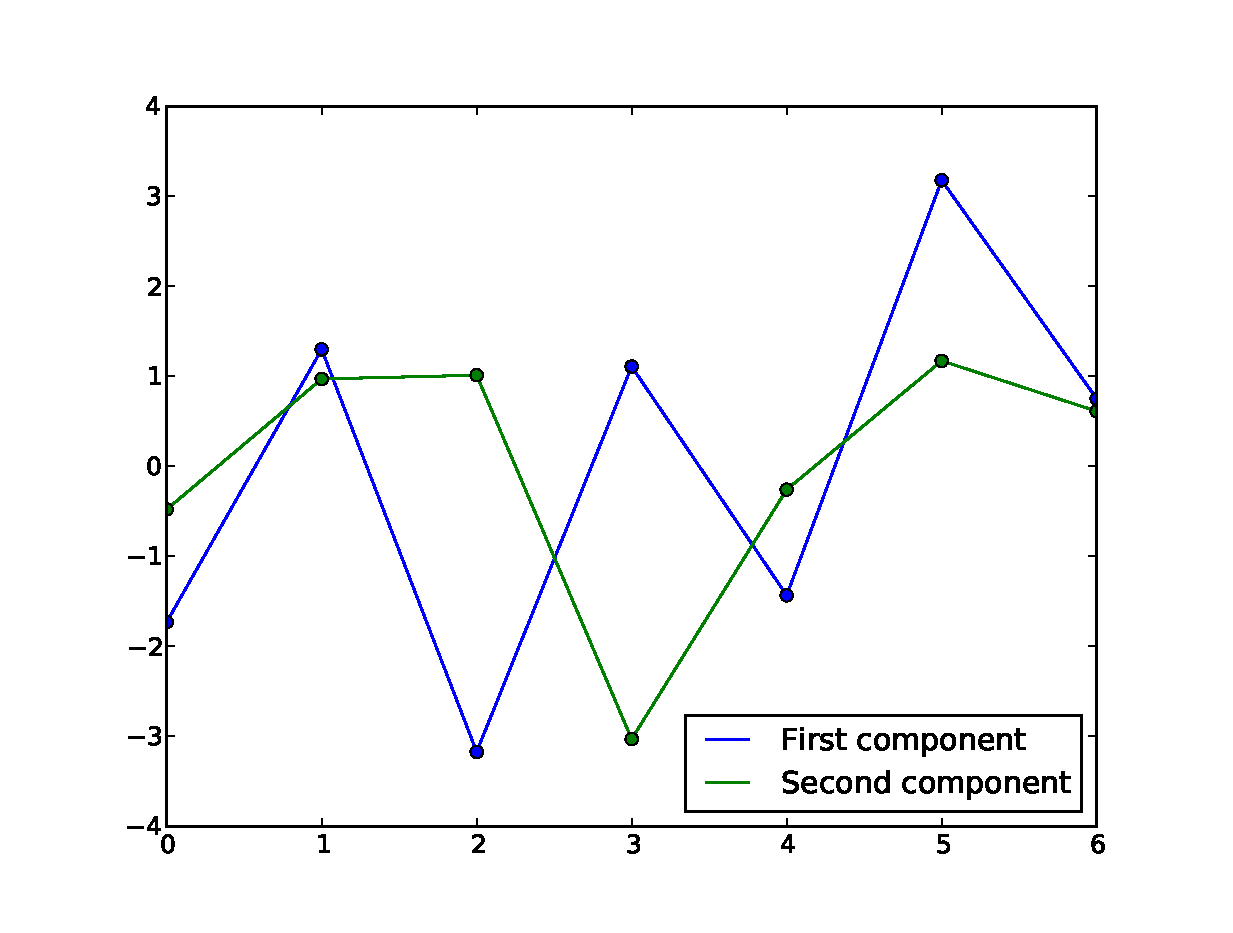
\includegraphics[width=0.45\textwidth]{images/g2filosofos}
%   \end{center}
%   \caption{\it Time evolution of the two principal components~\cite{Fabbri}.}
%   \label{fig:phitime}
% \end{figure}

The opposition and skewness indices for philosophers listed in Table
\ref{tab:tablephiOI}, endorse the minor role of opposition in
composers. We can note strong opposition and rather small skewness
on philosophical moves while small opposition and strong skewness on
musical moves. A fact that could explain the differences is the more
homogeneous distribution of scores on composers, while on philosophers
the scores shown significantly quantitative difference, concerning the
nature of their characteristics. 

\begin{table}%\footnotesize%\scriptsize%\tiny
\caption{\label{tab:tablephiOI}Opposition and skewness indices for each
of the six philosophical moves~\cite{Fabbri}.}

% \begin{ruledtabular}
\begin{tabular}{|c||c|c|}
\hline
Philosophical Move & $W_{i,j}$ & $s_{i,j}$ \\
\hline \hline
Plato $\rightarrow$ Aristotle &  1.0 & 0 \\
Aristotle $\rightarrow$ Descartes & 0.8622 & 0.8656 \\
Descartes $\rightarrow$ Espinoza & 0.9803 & 1.4930 \\
Espinoza $\rightarrow$ Kant & 0.5693 & 0.4715 \\
Kant $\rightarrow$ Nietzsche & 0.8021 & 0.8726 \\
Nietzsche $\rightarrow$ Deleuze & 0.3647 & 0.3148 \\
\hline
\end{tabular}
% \end{ruledtabular}
\end{table}

When comparing dialectics, other curious facts arise: the dialectics
indices on Table \ref{tab:tablephiE} are considerably stronger philosophical moves than for
composers. Both indices are also shown in Figure
\ref{fig:comparingdialectics} where we can see a constantly decrease
of counter-dialectics, contrasting the continuously variation of the
indices when considering the composers. This makes possible to argue
that dialectics is stronger on philosophy than on music where a
constantly return to the origins are clearly visible on some
composers. This reveals the nature of the
musical development, based on the search for a unity. Using the words
of Webern, the search for the ``comprehensibility'', but always
inheriting the teachings of their old masters.

\begin{table}%\footnotesize%\scriptsize%\tiny
\caption{\label{tab:tablephiE} Counter-dialectics index for each
of the five subsequent pairs of philosophical moves.}

\begin{tabular}{|c||c|}
\hline
Philosophical Triple & $d_{i \rightarrow k}$ \\
\hline \hline
Plato $\rightarrow$ Aristotle $\rightarrow$ Descartes &  0.700 \\
Aristotle $\rightarrow$ Descartes $\rightarrow$ Espinoza & 0.466 \\
Descartes $\rightarrow$ Espinoza $\rightarrow$ Kant & 0.137 \\
Espinoza $\rightarrow$ Kant $\rightarrow$ Nietzsche & 0.048 \\
Kant $\rightarrow$ Nietzsche $\rightarrow$ Deleuze  & 0.015 \\
\hline
\end{tabular}
% \end{ruledtabular}
\end{table}

\begin{figure}[ht]
        \begin{center}
                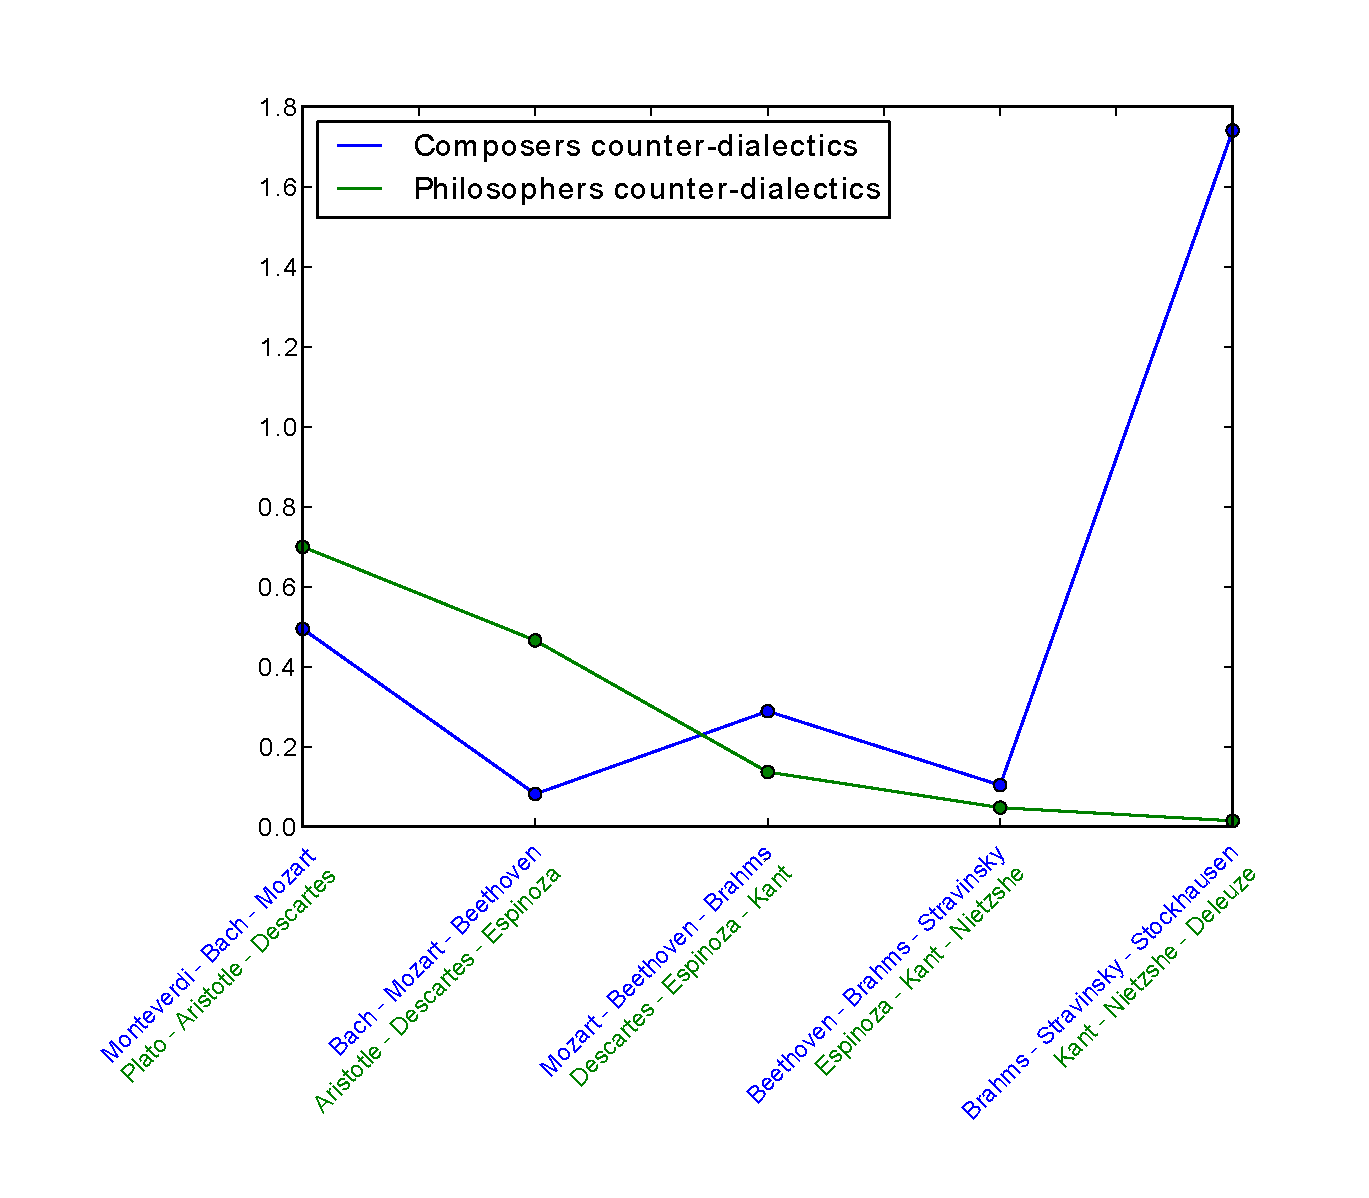
\includegraphics[width=0.45\textwidth]{images/compara_dialeticas2}
        \end{center}
        \caption{\it Comparison between composers and philosophers
          counter-dialectics indices}
        \label{fig:comparingdialectics}
\end{figure}

\section{Concluding Remarks}

Motivated by the understanding of how innovation on music history
evolves compared with philosophy, we extended a quantitative method
recently applied to the study of philosophical characteristics. Statistics
methods have been historically applied to the study of music features and
composers productivity, but not for the analysis of
composers characteristics. The method differs from the others on the
aspect of how the characteristics concerning composers are treated:
scores are attributed for each feature commonly noticeable on the
works of renowned composers. These scores reveals not the
exact profile of composers but a tendency of how their composition
techniques relate with each other. In order to investigate the
relationship between this scoring we applied Pearson correlation
analysis. The results demonstrated a strong correlation between the
characteristics, which allows us to group this values, creating a
reduced number of features that summarizes the most important
characteristics. PCA was also applied to these components, reducing
the complex space to a planar graph where the most interesting
properties were identified. 

Historical landmarks in  music are
well-defined on the graph, like the isolated geniuses of Bach and Mozart, the
proximity between Beethoven and Brahms, the heterogeneity of
Stravinsky or the vanguard of contemporary composers
like Stockhausen. Even not so visible relations, like the return to the
maximum domain of polyphony -- present on Renaissance -- by Beethoven
could also be clearly observable. 

The dichotomy between
master-apprentice tradition on music and the quest for innovation that
opened this discussion could be visualized quantitatively. Each
composer demonstrated his own style, differing considerably from his
predecessor -- clearly shown when analyzing pairs of subsequent composers like
Bach and Mozart, Mozart and Beethoven or Stravinsky and
Stockhausen. Otherwise, the inheritance of predecessors styles is also
present when analyzing the direct relations between Beethoven and
Brahms, or indirect ones between Bach and Beethoven
or Beethoven and Monteverdi. The entire scenario presented
a ``cyclical pattern'' between
composers -- motivated by the influence of theirs predecessors -- but also showed a force
repelling both of them: the innovation, or in the words of William
Lovelock, the ``experimentation'' that makes progress possible.

Along the analysis we noticed interesting differences when comparing
composers with philosophers. While on philosophy the
innovation is notably marked by opposition of each philosophers ideas,
it is less present for music composers. The lack of strong
opposition movements in musical space indicates the music innovation is driven by
a constant inheritance of each composer from his predecessors. We
represented this characteristic referring to a \textit{memory state}
where philosophers shows \textit{memory-2} -- each philosopher was
influenced by the opposite ideas of its two predecessors -- while
composers shows \textit{memory-1} -- inheriting the style of their direct
predecessor. 
The
analysis of both dialectics values also shown surprising
results: while on philosophy the dialectics indices are arranged on a
increasing series -- showing a strong influence of
dialectics to philosophy development -- the same dialectics indices on
music exhibits a constantly variation. This behavior presumably indicates a
constantly quest for coherence by the composers, a fact previously observed by
the studies of Anton Webern.

The quantitative methodology initially applied to the analysis of philosophy
proved to be extensible to other fields of knowledge like
music, reflecting with considerable efficiency, specific details
concerning each field. 
Computational analysis of music scores could be
applied to automate the quantification of composers characteristics, like
identification of melodic and harmonic patterns or the presence or not of
polyrhythms, motivic and harmonic stability~\cite{Correa}. More composers could be
inserted on the set for the analysis of a wider time-line, possibly
including more representatives of each music periods. 


While taking the first
steps on the direction of a quantitative approach to arts and philosophy
we believe that an understanding of the creative process could also
be eventually quantified. We want to end this work quoting Webern
again, who early envisioned these relations: ``It is clear that where relatedness and unity are omnipresent,
comprehensibility is also guaranteed. And all the rest is
dilettantism, nothing else, for all time, and always has been. That's
so not only in music but everywhere.''





%%%%%%%%% NOTAS %%%%%%%%%%%%%%%%%%%%%%%%%%%%%%%%%%%%%%%%%%%%%%%%%%%%

%oposição X inovação => quanto maior oposição, maior inovação?

% criatividade X coerência => coerência é derivada de tendências
%                             se olharmos para a árvore de tendências,
%                             o caminho que teve mais filhos possui
%                             maior coerência? conseguimos achar essa
%                             árvore quantitativamente? talvez
%                             clustering...

%                             coerência é associada a um objetivo.
%                             se o objetivo é expressar a música como
%                             um todo, harmonia e melodia 

% talvez a coerência limite dessa forma a criatividade, pois força a
% permanência em uma determinada tendência, limitando a
% experimentação. porém, pode-se ser criativo mesmo seguindo uma
% tendência e isso é visível nas diferenças entre os compositores, mesmo
% que quando seguindo os ensinamentos de seus mestres.

% novos espaços => analisar por tendências? separar por 

%\section{Relations with Computational Creativity}

% boden: composição, exploração & transformação

% indicar perspectivas quando se tratar de ligar com criatividade => arquitetura

% o que "dispara"/leva à criatividade? quais fatores?

\nocite{*}
\bibliography{musimetrics}

\end{document}
%
% ****** End of file aipsamp.tex ******
